%
% $RCSfile: paper.tex,v $
%
% Copyright (c) 2001-2004. Christian Heller. All rights reserved.
%
% Permission is granted to copy, distribute and/or modify this document
% under the terms of the GNU Free Documentation License, Version 1.1
% or any later version published by the Free Software Foundation;
% with no Invariant Sections, with no Front-Cover Texts and with no Back-Cover
% Texts. A copy of the license is included in the section entitled
% "GNU Free Documentation License".
%
% http://www.cybop.net
% - Cybernetics Oriented Programming -
%
% http://www.resmedicinae.org
% - Information in Medicine -
%
% @author Christian Heller <christian.heller@tuxtax.de>
% @author Jens Bohl <info@jens-bohl.de>
%

%
% The document class specifying the type of document.
%
\documentclass[a4paper,10pt]{llncs}

%
% The usepackages for document class.
%

% Paper format and font.
\usepackage{a4,times,helvet}

% Graphics.
\usepackage{graphicx}

%
% The space settings for edges (left, top, right, bottom).
%
\setlength{\hoffset}{-1,3in}
\setlength{\voffset}{-1in}
\setlength{\oddsidemargin}{3,5cm}
\setlength{\topmargin}{1,3cm}
%\setlength{\headwidth}{16,5cm}
\setlength{\headheight}{0cm}
\setlength{\textwidth}{16,5cm}
\setlength{\textheight}{23,2cm}

%
% The hyphenation list.
%
%
% $RCSfile: hyphenation.tex,v $
%
% Copyright (c) 2002-2007. Christian Heller. All rights reserved.
%
% Permission is granted to copy, distribute and/or modify this document
% under the terms of the GNU Free Documentation License, Version 1.1 or
% any later version published by the Free Software Foundation; with no
% Invariant Sections, with no Front-Cover Texts and with no Back-Cover
% Texts. A copy of the license is included in the section entitled
% "GNU Free Documentation License".
%
% http://www.cybop.net
% - Cybernetics Oriented Programming -
%
% Version: $Revision: 1.2 $ $Date: 2007-08-01 13:59:00 $ $Author: christian $
% Authors: Christian Heller <christian.heller@tuxtax.de>
%

\hyphenation{abs-trac-tion}
\hyphenation{ac-tu-ally}
\hyphenation{ana-lyst}
\hyphenation{ana-ly-sis}
\hyphenation{an-cient}
\hyphenation{ap-pli-ca-tion}
\hyphenation{aris-to-tle}
\hyphenation{at-tri-bute}
\hyphenation{be-ing}
\hyphenation{ca-te-go-ri-za-tion}
\hyphenation{client}
\hyphenation{com-po-nen-ti-za-tion}
\hyphenation{com-pu-ter}
\hyphenation{con-fi-gure}
\hyphenation{con-nec-ted}
\hyphenation{cy-ber-ne-tics}
\hyphenation{cyboi}
\hyphenation{cybol}
\hyphenation{cybop}
\hyphenation{des-cribed}
\hyphenation{de-sign}
\hyphenation{de-ve-lop-ment}
\hyphenation{dis-crete}
\hyphenation{di-vide}
\hyphenation{do-main}
\hyphenation{dy-na-mic}
\hyphenation{eli-mi-nate}
\hyphenation{eli-mi-nates}
\hyphenation{eli-mi-na-tion}
\hyphenation{en-gi-nee-ring}
\hyphenation{en-vi-ron-ment}
\hyphenation{ex-pert}
\hyphenation{fi-gure}
\hyphenation{fle-xi-bi-li-sie-rung}
\hyphenation{fun-da-men-tal}
\hyphenation{hard-ware}
\hyphenation{hu-man}
\hyphenation{im-ple-men-ta-tion}
\hyphenation{in-he-rit}
\hyphenation{in-he-ri-tance}
\hyphenation{in-ter-pre-ter}
\hyphenation{java}
\hyphenation{know-ledge}
\hyphenation{lan-guage}
\hyphenation{li-ving}
\hyphenation{lo-gi-cal}
\hyphenation{ma-na-ge-ment}
\hyphenation{mea-ning-ful}
\hyphenation{me-cha-nism}
\hyphenation{me-mo-ry}
\hyphenation{me-thod}
\hyphenation{me-thods}
\hyphenation{mo-del-ling}
\hyphenation{na-ture}
\hyphenation{net-work}
\hyphenation{neu-ral}
\hyphenation{neu-ron}
\hyphenation{ne-ver-en-ding-ly}
\hyphenation{open}
\hyphenation{operating}
\hyphenation{ori-en-ted}
\hyphenation{over-come}
\hyphenation{par-ti-cu-lar}
\hyphenation{prin-ci-ple}
\hyphenation{pro-ba-bi-lis-tic}
\hyphenation{pro-ble-ma-tic}
\hyphenation{pro-gram-ming}
\hyphenation{res-pon-sible}
\hyphenation{re-u-sa-bi-li-ty}
\hyphenation{sci-ence}
\hyphenation{server}
\hyphenation{si-mi-lar}
\hyphenation{soft-ware}
\hyphenation{source}
\hyphenation{spe-cia-li-za-tion}
\hyphenation{spe-ci-fied}
\hyphenation{sta-tic}
\hyphenation{sta-ti-cally}
\hyphenation{sto-chas-tic}
\hyphenation{stone-on-stone}
\hyphenation{struc-ture}
\hyphenation{strug-gling}
\hyphenation{subs-ti-tu-ting}
\hyphenation{su-per-flu-ous}
\hyphenation{sup-ply-ing}
\hyphenation{sys-tem}
\hyphenation{taeu-schungs-ver-such}
\hyphenation{temp-lates}
\hyphenation{tes-ting}
\hyphenation{thin-king}
\hyphenation{un-en-li-vened}
\hyphenation{un-sa-tis-fy-ing}
\hyphenation{va-ry-ing}
\hyphenation{weigh-ted}
\hyphenation{zu-kunfts-si-che-re}


%
% This document is a scientific paper to be handed in for a conference.
%
% @version $Revision: 1.3 $ $Date: 2003-05-19 08:49:57 $ $Author: christian $
% @author Christian Heller <christian.heller@tuxtax.de>
% @author Christian Heller <christian.heller@tu-ilmenau.de>
%
\begin{document}
    \twocolumn
    \title{Flexible Software Architectures for Presentation Layers demonstrated on Medical Documentation with Episodes and Inclusion of Topological Report}
\author{Jens Bohl \(<\)info@jens-bohl.de\(>\)\\
Torsten Kunze \(<\)zone3@gmx.de\(>\)\\
Christian Heller \(<\)christian.heller@tu-ilmenau.de\(>\)\\
Ilka Philippow \(<\)ilka.philippow@tu-ilmenau.de\(>\)}
\institute{
Technical University of Ilmenau\\
Faculty for Computer Science and Automation\\
Institute for Theoretical and Technical Informatics\\
PF 100565, Max-Planck-Ring 14, 98693 Ilmenau, Germany\\
http://www.tu-ilmenau.de, fon: +49-(0)3677-69-1230, fax: +49-(0)3677-69-1220}
\maketitle

    \maketitle
    %
% $RCSfile: abstract.tex,v $
%
% Copyright (c) 2001-2004. Christian Heller. All rights reserved.
%
% No copying, altering, distribution or any other actions concerning this
% document, except after explicit permission by the author!
% At some later point in time, this document is planned to be put under
% the GNU FDL license. For now, _everything_ is _restricted_ by the author.
%
% http://www.cybop.net
% - Cybernetics Oriented Programming -
%
% http://www.resmedicinae.org
% - Information in Medicine -
%
% @author Christian Heller <christian.heller@tuxtax.de>
%

\begin{abstract}
This article reports about an ongoing research investigating the possibilities
for applying inter-disciplinary concepts to software system design. The new
resulting programming philosophy is based on firstly, a distinction of statics
and dynamics, secondly a knowledge schema structuring models and their meta
information hierarchically, and thirdly the separation of state- and logic
knowledge. It solves many of the problems existing in classical programming
paradigms and languages and may have the potential to replace these in the long
run.\\
\textbf{Keywords:} Knowledge Abstraction, Cybernetics Oriented Programming,
CYBOP, Software Design
\end{abstract}

    \section{Introduction}
Quality of software is often defined by its maintainability,
extensibility and flexibility. \emph{Object Oriented Programming} (OOP)
should help to achieve these goals -- but this wasn't possible by only
introducing another programming paradigm.\\
So, major research objectives are to find concepts and principles
to increase the reusability of software architectures and the
resulting code. \emph{Frameworks} shall prevent code duplication and
development efforts. Recognizing recurring structures means finding
\emph{Design Patterns} for application on similar problems. These two
concepts -- frameworks and design patterns -- depend on each other
and provide a higher flexibility of software components \cite{ch:pree}.\\
The aim of this work was to find suitable combinations of design
patterns to compose a framework that is characterized by a strict
hierarchical architecture. Everything in universe is organized
within a hierarchy of elements -- the human body for example
consists of organs, organs consist of regions, regions consist of
cells and so on. This very simple idea can also be mapped on
software architectures -- and basically, this is what this document
is about.\\
What kind of techniques to realize such a concept of strict
hierarchy does software engineering provide? The following
chapters first introduce common design patterns and the lifecycle
of components as templates for own ideas and then show how the
resulting framework \emph{Cybernetics Oriented Programming}
(CYBOP) \cite{cybop} is designed.

    %
% $RCSfile: state.tex,v $
%
% Copyright (c) 2001-2004. Christian Heller. All rights reserved.
%
% Permission is granted to copy, distribute and/or modify this document
% under the terms of the GNU Free Documentation License, Version 1.1
% or any later version published by the Free Software Foundation;
% with no Invariant Sections, with no Front-Cover Texts and with no Back-Cover
% Texts. A copy of the license is included in the section entitled
% "GNU Free Documentation License".
%
% http://www.cybop.net
% - Cybernetics Oriented Programming -
%
% http://www.resmedicinae.org
% - Information in Medicine -
%
% @author Christian Heller <christian.heller@tuxtax.de>
% @author Jens Bohl <info@jens-bohl.de>
%

\section{Design Principles}
\label{design_principles_heading}

\subsection{Essential Design Patterns}
\label{essential_design_patterns_heading}

Design patterns \cite{gamma1995} are elements of reusable software. They can be
used for solving recurrent design problems and are recommendations on how to build
software in an elegant way. With the help of these patterns, software shall be
more extensible, flexible and easy to maintain with respect to future enhancements.
The following patterns are essential within CYBOP.

\subsubsection{Composite}
\label{composite_heading}

This design pattern (figure \ref{composite_figure}) allows creating tree-like
object structures. One object is child of another object and has exactly one
parent. This pattern is often used to realize \emph{Whole-Part} relations:
one object is \emph{Part} of another one.

\begin{figure}[ht]
    \begin{center}
       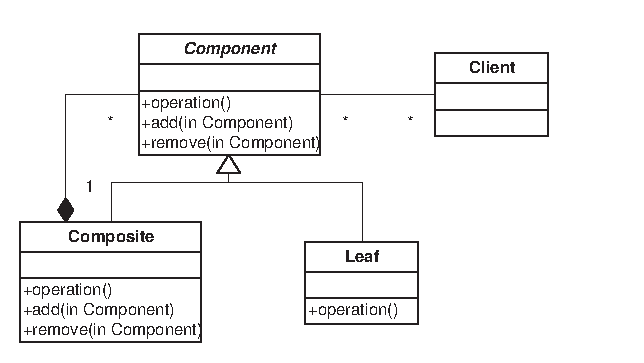
\includegraphics[scale=0.7]{eps/compositum.eps}
       \caption{Composite Pattern}
       \label{composite_figure}
    \end{center}
\end{figure}

\subsubsection{Layers}
\label{layers_heading}

With the help of this pattern, software can be organized in horizontal layers
(figure \ref{layer_figure}). Modules and applications can be separated into logical
levels, whereby these levels should be as independent from each other as possible,
to ensure a high substitutability.

\begin{figure}[ht]
    \begin{center}
       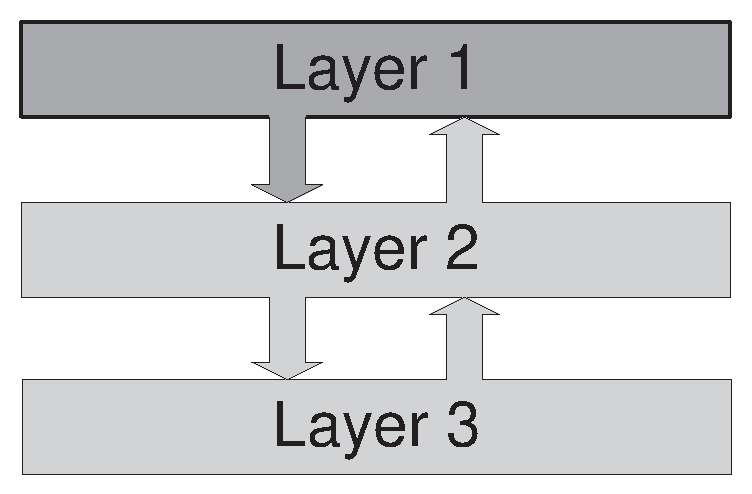
\includegraphics[scale=0.5]{eps/3-Tier-1.eps}
       \caption{Layer Pattern}
       \label{layer_figure}
    \end{center}
\end{figure}

\subsubsection{Chain Of Responsibility}
\label{chain_of_responsibility_heading}

Messages initiated by a particular object can be sent over a chain of instances
to the receiving object (figure \ref{chain_of_responsibility_figure}). So, either
the message will be transmitted over a bunch of objects or evaluated immediately
by the target object.

\begin{figure}[ht]
    \begin{center}
       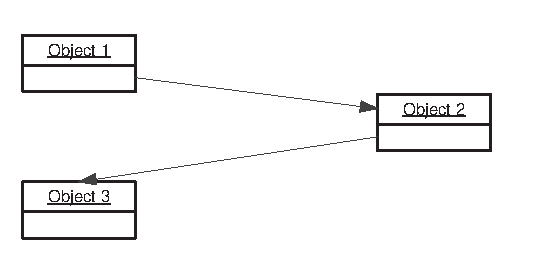
\includegraphics[scale=0.8]{eps/chain.eps}
       \caption{Chain Of Responsibility Pattern}
       \label{chain_of_responsibility_figure}
    \end{center}
\end{figure}

\subsubsection{Model-View-Controller}
\label{model_view_controller_heading}

Dividing the presentation layers into the logical components \emph{Model},
\emph{View} and \emph{Controller}, is a very approved way for designing software
for user interfaces. The model encapsulates the data presented by the view and
manipulated by the controller (figure \ref{model_view_controller_figure}).

\begin{figure}[ht]
    \begin{center}
       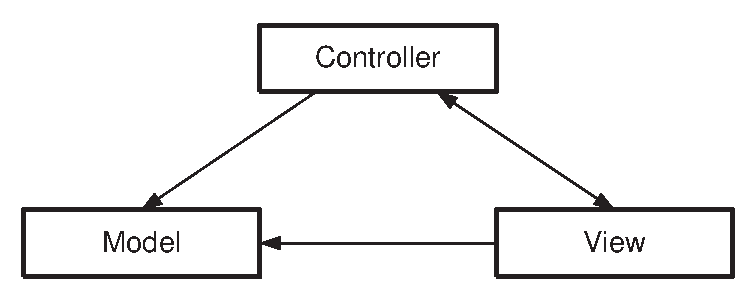
\includegraphics[scale=0.6]{eps/mvc-1.eps}
       \caption{Model-View-Controller Pattern}
       \label{model_view_controller_figure}
    \end{center}
\end{figure}

\subsubsection{Hierarchical Model-View-Controller}
\label{hierarchical_model_view_controller_heading}

The Hierarchical Model-View-Controller \cite{cai} combines the essential design
patterns \emph{Composite}, \emph{Layers} and \emph{Chain of Responsibility}
into one conceptual architecture (figure \ref{hierarchical_model_view_controller_figure}).
This architecture divides the presentation layer into hierarchical sections
containing \emph{MVC-Triads}. The triads conventionally consist of model, view
and controller parts. Triads communicate with each other by relating over their
controller object.\\
Here is a short explanation of this concept, using a practical example:
The upper-most triad could represent a dialog and the middle one a container
such as a panel. In this container, a third triad -- for example a button --
could be held.

\begin{figure}[ht]
    \begin{center}
       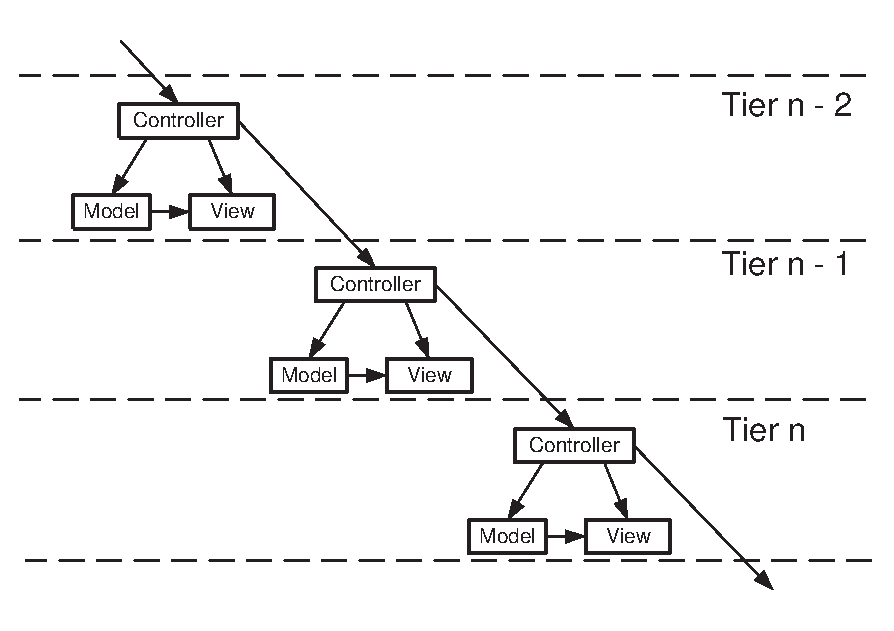
\includegraphics[scale=0.5]{eps/hmvc.eps}
       \caption{Hierarchical Model-View-Controller Pattern}
       \label{hierarchical_model_view_controller_figure}
    \end{center}
\end{figure}

\subsection{Component Lifecycle}
\label{component_lifecycle_heading}

Each \emph{Component} lives in a system that is responsible for the component's
creation, destruction etc. When talking about components, this article sticks
to the definition of Apache-Jakarta-Avalon \cite{jakarta}, which considers
components to be \emph{a passive entity that performs a specific role}.\\
A component has a number of methods which need to be called in a certain order.
The order of method calls is what is known as \emph{Component Lifecycle}.
An outside, active entity is responsible for calling the lifecycle methods
in the right order. In other words, such an entity or \emph{Component Container}
can control and use the component. The Avalon documentation \cite{jakarta} says:

\begin{quotation}
    \textit{
        It is up to each container to indicate which lifecycle methods it will honor.
        This should be clearly documented together with the description of the container.
    }
\end{quotation}


    \section{An Extended Component Lifecycle}

The CYBOP lifecycle of components is an extension of the lifecycle idea of Apache
-- basically the same idea but another background and realization.\\
All \emph{whole-part associations} between objects were organized
under the rules of the component lifecycle. Analogous to the
lifecycle of organic cells, the relations were created and
destroyed in a sequence of lifecycle steps. These steps are
realized as method calls on the components (see figure \ref{State
Diagram of CYBOB's Component Lifecycle}).
\includepicture{8}{eps/lebenszyklusEng.eps}{State Diagram of CYBOB's Component Lifecycle}{State Diagram of CYBOB's Component Lifecycle}{State Diagram of CYBOB's Component Lifecycle} {State Diagram of CYBOB's Component Lifecycle}

    %
% $RCSfile: ontology.tex,v $
%
% Copyright (c) 2001-2004. Christian Heller. All rights reserved.
%
% No copying, altering, distribution or any other actions concerning this
% document, except after explicit permission by the author!
% At some later point in time, this document is planned to be put under
% the GNU FDL license. For now, _everything_ is _restricted_ by the author.
%
% http://www.cybop.net
% - Cybernetics Oriented Programming -
%
% http://www.resmedicinae.org
% - Information in Medicine -
%
% @author Christian Heller <christian.heller@tuxtax.de>
%

\subsection{Ontology}
\label{ontology_heading}

Manifold definitions of the word \emph{Ontology} exist. They come from philosophy,
metaphysics, information technology and others -- too many to list here.
This document uses its own, adapted definition and considers an ontology to be
\emph{a strict hierarchy of abstract items, organized in levels of growing
granularity, that are solely unidirectionally related}. It such represents a
systematic description of complex domain contexts.

\begin{figure}[ht]
    \begin{center}
        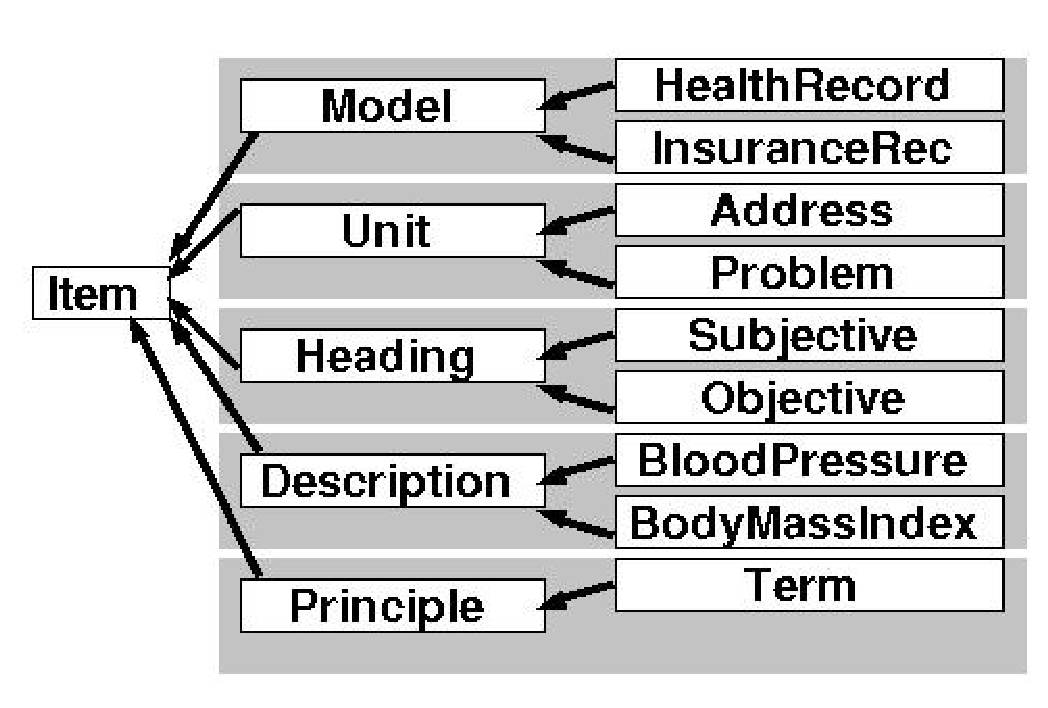
\includegraphics[scale=0.4]{vector/electronic_health_record_ontology.eps}
        \caption{Electronic Health Record Ontology}
        \label{electronic_health_record_ontology_figure}
    \end{center}
\end{figure}

Figure \ref{electronic_health_record_ontology_figure} shows one possible ontology
of an electronic health record, as described in the previous section.


    %
% $RCSfile: framework.tex,v $
%
% Copyright (C) 2002-2008. Christian Heller.
%
% Permission is granted to copy, distribute and/or modify this document
% under the terms of the GNU Free Documentation License, Version 1.1 or
% any later version published by the Free Software Foundation; with no
% Invariant Sections, with no Front-Cover Texts and with no Back-Cover
% Texts. A copy of the license is included in the section entitled
% "GNU Free Documentation License".
%
% http://www.cybop.net
% - Cybernetics Oriented Programming -
%
% http://www.resmedicinae.org
% - Information in Medicine -
%
% Version: $Revision: 1.1 $ $Date: 2008-08-19 20:41:06 $ $Author: christian $
% Authors: Christian Heller <christian.heller@tuxtax.de>
%

\subsection{Framework}
\label{framework_heading}
\index{Framework}
\index{Software Framework}
\index{Pattern}
\index{Base Architecture}
\index{Library}
\index{Callback Mechanism}
\index{Inheritance}
\index{Polymorphism}
\index{Static Constraints of a Framework}
\index{Dynamic Parts of a Framework}
\index{Frozen Spot}
\index{Hot Spot}
\index{Contract}
\index{Vertical Market Framework}
\index{Horizontal Market Framework}
\index{Java Development Kit}
\index{JDK}
\index{Collection Framework}
\index{Input Method Framework}
\index{Bidirectional Dependency}
\index{Observer Pattern}
\index{Manager Class}
\index{Singleton Pattern}

In the past decade, \emph{Software Frameworks} have gained in importance.
Patterns are considered their elementary building blocks. Yet while patterns
are solutions for recurring design problems, frameworks represent the base
architecture for a family of systems \cite{pree}. Because both concepts depend
on each other, frameworks are described within the main section \emph{Patterns}.

A \emph{Framework} essentially is a reusable collection of a number of
cooperating abstract and concrete classes, in a special constellation. It
represents an imcomplete software system which still needs to be extended and
instantiated, to be executable. A conventional \emph{Library} is used by
calling the procedures provided by it; the main part of each application is
then designed and realised by the developer. A \emph{Framework} already
represents the actual main part of a system. Functionality added by the
application developer is reversely called and used by the framework itself.
This principle carries the name \emph{Callback Mechanism}. Extensions are
mostly realised through \emph{Inheritance} and \emph{Polymorphism} (section
\ref{object_oriented_programming_heading}).

But not all parts of a framework are intended to be extended. After W. Pree
\cite{pree}, there are \emph{Static Constraints} and \emph{Dynamic Parts}.
Buschmann \cite{buschmann} calls them \emph{Frozen Spots} and \emph{Hot Spots};
the \emph{Apache Jakarta Avalon} framework \cite{avalon} labels static parts
\emph{Contracts}. When the abstract state of a framework is turned into a
functioning application by instantiating its classes, static elements remain
unchanged. They form the basic structure for all derived applications.
Application-specific behaviour, on the other hand, is determined by
specialising adaptable framework parts.

The \emph{Jakarta Avalon} documentation \cite{avalon} defines a framework as:

\begin{enumerate}
    \item A supporting or enclosing structure.
    \item A basic system or arrangement as of ideas.
\end{enumerate}

It distinguishes between \emph{Vertical Market Frameworks} which focused on a
single industry like medical systems or telecommunications and would not work
well in other industries, and \emph{Horizontal Market Frameworks} which were
generic enough to be used across multiple industries. Vertical market frameworks
could be built on top of horizontal market frameworks.

Just like patterns, frameworks provide higher flexibility to software components,
prevent code duplication and lower development efforts \cite{pree}. Developers
are freed from frequently reinventing the same solutions and can concentrate on
actual application development. The similar structure of applications that base
on the same framework ensures consistency and eases their maintenance, and also
reduces the time it takes for a developer to learn how the software works. Of
course, the necessary adjustment for new developers should not be underestimated;
comprehensive documentation is necessary. But once the principles behind a
framework are understood, one will be able to comprehend any system built upon it.

The \emph{Java Development Kit} (JDK) \cite{java}, for example, offers a number of
special \emph{Collection} containers (section \ref{container_heading}) which it
calls \emph{Collection Framework}; there is also an \emph{Input Method Framework}
and so on. Over the years, however, the framework definition has become a bit
fuzzy here-and-there.

The price of framework reusability is \emph{Lower Flexibility}, which is due to
the above-mentioned static parts. Besides this, applications are subject to the
evolution of the underlying framework. However, that disadvantage shouldn't be
too bold, if the framework is designed general and clever enough.

Framework callback mechanisms rely on \emph{Bidirectional Dependencies} and bring
with all their disadvantages (section \ref{bidirectional_dependency_heading}). To
explain this briefly: Instances that want to be called by the framework need to
register at a caller before, as was explained in section \ref{observer_heading},
on the example of the \emph{Observer} pattern. In order to be able to register
themselves, callees need to know about the caller. Once callees are registered,
the caller knows about them in turn.

Frequently, statically accessible classes, also called \emph{Managers}, have to
be introduced to a framework, mostly due to unforeseen requirements. They often
use the \emph{Singleton} pattern (section \ref{singleton_heading}) to become
unique within a system. Managers of that kind serve as gateway to certain areas
of the framework that are not easily reachable anymore through normal navigation
along object associations. A number of negative effects related to static object
access were already mentioned (section \ref{global_access_heading}).

Chapter \ref{knowledge_schema_heading} introduces a structure called
\emph{Knowledge Schema} which, although being static, is capable of
representing general knowledge, thus allowing the creation of flexible
application systems. Bidirectional dependencies and global model (object)
access are not an issue in the new language and interpreter introduced in
chapters \ref{cybernetics_oriented_language_heading} and
\ref{cybernetics_oriented_interpreter_heading}, because any runtime knowledge
model may be accessed along well-defined paths in a simple tree-like structure.

    \section{Record -- An EHR Module}
The practical background for the application of CYBOP is \emph{Res Medicinae}.
A modern clinical information system is the aim of all efforts in this project.
In future, it shall serve medical documentation, archiving, laboratory work etc.
\emph{Res Medicinae} is separated into single modules depending on different tasks.\\
One of these modules is \emph{Record} -- an application for
documenting medical information (see figure \ref{Screenshot of
Record}). In addition to new documentation models,
it also contains a tool for topological documentation.\\
Starting from an over-all view of the human body, it is possible
to reach every organ or region of the body in detail (see figure
\ref{Excerpt from Topological Structure of Human Skeleton}).
\includepicture{6}{eps/screenshot.eps}{Screenshot of Record}{Screenshot of Record \cite{urban}}{Screenshot of Record}{Screenshot of Record}
\includepicture{6}{eps/topology.eps}{Excerpt from Topological Structure of Human Skeleton}{Excerpt from Topological Structure of Human Skeleton \cite{urban}}{Excerpt from Topological Structure of Human Skeleton}{Excerpt from Topological Structure of Human Skeleton}

    %
% $RCSfile: summary.tex,v $
%
% Copyright (c) 2001-2004. Christian Heller. All rights reserved.
%
% No copying, altering, distribution or any other actions concerning this
% document, except after explicit permission by the author!
% At some later point in time, this document is planned to be put under
% the GNU FDL license. For now, _everything_ is _restricted_ by the author.
%
% http://www.cybop.net
% - Cybernetics Oriented Programming -
%
% http://www.resmedicinae.org
% - Information in Medicine -
%
% @author Christian Heller <christian.heller@tuxtax.de>
%

\section{Summary}
\label{summary_heading}

This paper means that wild \emph{Dependencies} are a major reason for error-prone,
unstable, unflexible, unmaintainable software systems. Two facts causing such
dependencies are the \emph{Bundling} of static and dynamic properties by
object-oriented languages and the \emph{Mix} of knowledge and hardware control
in traditional programming languages. This information mix additionally forces
software development projects to run through a course of different abstraction
steps which would not differ if one common knowledge abstraction were used.

As solution to the above's problems, this document suggests to build software
systems after the concepts of \emph{Human Thinking}. The approach, named CYBOP,
such follows the recommendations of the science of \emph{Cybernetics} and its
specialization \emph{Bionics}, whereby biological principles should be applied
to the study and design of engineering systems. An abstract model as formed in the
human mind represents an \emph{Item}, \emph{Category} and \emph{Compound}, at the
same time. Additionally, it contains \emph{Meta Information} about its parts.
This information often corresponds to physical dimensions and determines whether
the model is an abstraction of \emph{static} or \emph{dynamic} real-world aspects.

The introduced \emph{CYBOL} language has the semantics to express knowledge models
as used by human thinking. It allows to create complete application systems. Its
syntax is based on \emph{XML} which results in absolutely platform- independent
system definitions. CYBOL files get interpreted by the \emph{CYBOI} interpreter
and can be changed at runtime. CYBOI manages all hardware access. It concentrates
model instances and signal handling in one place and such avoids memory leaks and
endless loops.

CYBOL models could be displayed graphically, using special design tools. But their
\emph{formal definition} also allows them to be used as main abstraction throughout
all phases in a software project's lifetime. Analysts and experts can start their
work by creating rudimentary CYBOL models (defining static structures and dynamic
processes) which software designers can later complete and check for correctness.
The implementation phase becomes superfluous at all: CYBOL models already represent
the system to be built, no further code is needed! It is hard to imagine the amount
of saved time and costs for software projects. Even better: Experts are placed in
a position to, themselves, actively help creating systems.

    %
% $RCSfile: acknowledgements.tex,v $
%
% Copyright (C) 2002-2008. Christian Heller.
%
% Permission is granted to copy, distribute and/or modify this document
% under the terms of the GNU Free Documentation License, Version 1.1 or
% any later version published by the Free Software Foundation; with no
% Invariant Sections, with no Front-Cover Texts and with no Back-Cover
% Texts. A copy of the license is included in the section entitled
% "GNU Free Documentation License".
%
% http://www.cybop.net
% - Cybernetics Oriented Programming -
%
% http://www.resmedicinae.org
% - Information in Medicine -
%
% Version: $Revision: 1.1 $ $Date: 2008-08-19 20:41:05 $ $Author: christian $
% Authors: Christian Heller <christian.heller@tuxtax.de>
%

\section*{Acknowledgements}
\label{acknowledgements_heading}
%\addcontentsline{toc}{section}{Acknowledgements}

Certainly, first thanks is due my wife \emph{Kasia} and my \emph{Parents} and
\emph{Sisters}, being always with me, in good as in bad times. Not less
important to me are my aunt \emph{Maria Kosiza}, my great \emph{Relatives} and
our former chaplain \emph{Johannes Preis}, who have helped shaping me the way I
am.

I would like to thank my professor, \emph{Ilka Philippow}, for greatly
encouraging me during my work while leaving enough room to develop my own
ideas. Equal thanks is due my supervisors \emph{Dietrich Reschke} and
\emph{Mark Lycett}. \emph{Detlef Streitferdt} and \emph{Bernd D\"ane} gave
numerous hints improving the quality of the first part of my work. Consultation
with Bernd and \emph{Wolfgang Fengler} helped me understand Petri Net diagrams
and their hardware background as well as Assembler programming. Whenever I
got doubts about what I was doing, I was very lucky to receive good motivation
from my colleagues \emph{Volker Langenhan}, \emph{Oswald Kowalski},
\emph{Todor Vangelov} and \emph{Kai B\"ollert}. Oswald's talks about hardware
concepts made me find useful parallels to software. Alexander Fleischer helped
out when I was struggling with \LaTeX's paper size option.

My thanks go to my students \emph{Jens Bohl}, \emph{Torsten Kunze},
\emph{Dirk Behrendt}, \emph{Kumanan Kanagasabapathy}, \emph{Jens Kleinschmidt},
\emph{Martin Fache}, \emph{Karsten Tellhelm}, \emph{Marcel Kiesling},
\emph{Teodora Kikova}, \emph{Dennis Reichenbach}, \emph{Stefan Zeisler},
\emph{Michael Simon}, \emph{Henrik Brandes} and \emph{Saddia Malik} for
contributing their theses, tutorials or source code to the project. Special
thanks to \emph{Rolf Holzm\"uller} who brought in some innovative ideas for
CYBOL, in the final phase of my work, and helped cleaning many bugs in CYBOI.

Reminiscences on good times go to my former colleagues of \emph{OWiS Software}
who, together with the \emph{Technical University of Ilmenau} (TUI), have
contributed with great commitment to the development of the
\emph{Object Technology Workbench} (OTW) UML tool which I would have liked to
use in the early stages of my work. Pity it hasn't gone Open Source after its
development was stopped in 2000 :-( Thanks to \emph{Martin Wolf},
\emph{Rene Prei\ss{}el}, \emph{Dirk Henning} and all colleagues who have been
patient and well-explaining teachers!

I would like to acknowledge the contributors of \emph{CYBOP} \cite{cybop} and
\emph{Res Medicinae} \cite{resmedicinae}, especially all medical doctors, e.g.
\emph{Claudia Neumann} and \emph{Karsten Hilbert}, who supported the second
project with their analysis work \cite{resmedicinae2001} and mailing list
discussions. Furthermore, I want to mention \emph{Thomas Beale} from the
\emph{OpenEHR} project \cite{openehr} whose freely published design document
(back in 2001) gave me some initial ideas in the early stage of my work.
Acknowledged be all these brave \emph{Enthusiasts} of the
\emph{Free/ Libre Open Source Software} (FLOSS) community, who have provided me
with a great amount of knowledge through a comprising code base to build on.
I shall mention the contributors of FLOSS projects such as \emph{Scope}
\cite{scope}, \emph{Apache Jakarta} \cite{jakarta}, \emph{JOS} \cite{jos},
\emph{JDistro} \cite{jdistro}, the \emph{OpenHealth} \cite{openhealth} mailing
list readers, the \emph{OSHCA} \cite{oshca} members and all other supporters of
our projects and ideals.

Great thanks goes to the \emph{Urban und Fischer} publishing company, for
providing anatomical images from their \emph{Sobotta: Atlas der Anatomie}
\cite{urban} and to the \emph{Open Clip Art} project \cite{openclipart} for its
wonderful library of free art! Similarly, I have to thank the free online
dictionaries of \emph{LEO} \cite{leo} and the
\emph{Technical University of Chemnitz} \cite{tuchemnitz}.

I am grateful to all people who openly publish their knowledge on the web.
Without the numerous free sources, I would have never been able to accomplish
this work. Especially in the state-of-the-art part, I had to heavily rely on
existing sources. It is also therefore that I have decided to put my work under
the \emph{GNU FDL} licence \cite{gnulicences}. I would be happy to see large
parts of it copied in \emph{Wikipedia} \cite{wikipedia}!

    \label{references_heading}
    \bibliographystyle{geralpha}
    \bibliography{references}
\end{document}

